\documentclass[10.5pt,compsoc]{TsT}
\usepackage{graphicx}
\usepackage{footmisc}
\usepackage{subfigure}
\usepackage{url}
\usepackage{multirow}
\usepackage[noadjust]{cite}
\usepackage{amsmath,amsthm}
\usepackage{amssymb,amsfonts}
\usepackage{booktabs}
\usepackage{color}
\usepackage{ccaption}
\usepackage{booktabs}
\usepackage{float}
\usepackage{fancyhdr}
\usepackage{caption}
\usepackage{xcolor,stfloats}
\usepackage{comment}
\setcounter{page}{1}
\graphicspath{{figures/}}
\usepackage{cuted}  %flushend,
\usepackage{captionhack}
\usepackage{epstopdf}
%\usepackage[lite,subscriptcorrection,slantedGreek,nofontinfo]{mtpro2}

%===============================%
\headevenname{\zihao{-5}{\textbf{\emph{Tsinghua Science and Technology, June}}} 2013, 18(3): 000-000}%
\headoddname{{\sf Wang Zhenyang et al.:}\quad {\textbf{\emph{Attention to Difficulty: A Cascade Coarse to Fine Network Architecture for Semantic Segmentation}}}}%
%footnote use of *
\renewcommand{\thefootnote}{\fnsymbol{footnote}}
\newcommand{\upcite}[1]{\superscript{\textsuperscript{\cite{#1}}}}
\setcounter{footnote}{0}
\renewcommand\footnotelayout{\normalsize}

\newtheoremstyle{mystyle}{0pt}{0pt}{\normalfont}{1em}{\bf}{}{1em}{}
\theoremstyle{mystyle}
\renewcommand\figurename{Fig.~}
\renewcommand{\thesubfigure}{(\alph{subfigure})}
\newcommand{\upcite}[1]{\textsuperscript{\cite{#1}}}
\renewcommand{\labelenumi}{(\arabic{enumi})}
\newcommand{\tabincell}[2]{\begin{tabular}{@{}#1@{}}#2\end{tabular}}
\newcommand{\abc}{\color{white}\vrule width 2pt}


\newtheorem{assumption}{\textbf{Assumption}}
\newtheorem{definition}{\textbf{Definition}}
\newtheorem{lemma}{\textbf{Lemma}}
\newtheorem{theorem}{\textbf{Theorem}}
\newtheorem{proposition}{\textbf{Proposition}}
\newtheorem{corollary}{\textbf{Corollary}}






%\newcommand{\TODO}[1]{\textbf{TODO: #1}}

\addtolength{\abovecaptionskip}{-2mm}
\addtolength{\belowcaptionskip}{-2mm}

%%% aanpassing van cite aan journal style
\makeatletter
%\def\@cite#1#2{\textsuperscript{[{#1\if@tempswa, #2\fi}]}}
\renewcommand{\@biblabel}[1]{[#1]\hfill}
\makeatother

\begin{document}

\thispagestyle{empty}



\hyphenpenalty=50000

\makeatletter
\newcommand\mysmall{\@setfontsize\mysmall{7}{9.5}}

%%%%%%%%%%%%%%%%%%%%%%%
\newenvironment{tablehere}
  {\def\@captype{table}}
  {}
\newenvironment{figurehere}
  {\def\@captype{figure}}
  {}
%%%%%%%%%%%%%%%%%%%%%%%
%%%%%%%%%%%%%%%%%%%%%%%%%%%%%%%%

\thispagestyle{plain}%
\thispagestyle{empty}%

\let\temp\footnote
\renewcommand \footnote[1]{\temp{\zihao{-5}#1}}
{}
\vspace*{-40pt}

%{\hbox
\noindent{\zihao{5-}\textbf{\scalebox{0.89}[1.0]{\makebox[5.6cm][s]{%
TSINGHUA SCIENCE AND TECHNOLOGY}}}}

\vskip .2mm
{\zihao{5-}
\textbf{
\hspace{-5mm}
\scalebox{1}[1.0]{\makebox[5.6cm][s]{%
I\hspace{0.70pt}S\hspace{0.70pt}S\hspace{0.70pt}N\hspace{0.70pt}{\color{white}%
l\hspace{0.70pt}l\hspace{0.70pt}}1\hspace{0.70pt}0\hspace{0.70pt}0\hspace{0.70pt%
}7\hspace{0.70pt}-\hspace{0.70pt}0\hspace{0.70pt}2\hspace{0.70pt}1\hspace{0.70pt%
}4\hspace{0.70pt}{\color{white}l\hspace{0.70pt}l\hspace{0.70pt}}0\hspace{0.70pt}%
?\hspace{0.70pt}/\hspace{0.70pt}?\hspace{0.70pt}?\hspace{0.70pt}{\color{white}%
l\hspace{0.70pt}l\hspace{0.70pt}}p\hspace{0.70pt}p\hspace{0.70pt}?\hspace{0.70pt}?\hspace{0.70pt}?%
-\hspace{ 0.70pt}?\hspace{0.70pt}?\hspace{0.70pt}?}}}

\vskip .2mm\noindent
{\zihao{5-}\textbf{\scalebox{1}[1.0]{\makebox[5.6cm][s]{%
V\hspace{0.8pt}o\hspace{0.8pt}l\hspace{0.8pt}u\hspace{0.8pt}m\hspace{0.8pt}%
e\hspace{0.6em}1\hspace{0.8pt}8,\hspace{0.6em}N\hspace{0.8pt}u\hspace{0.8pt}%
m\hspace{0.8pt}b\hspace{0.8pt}e\hspace{0.8pt}r\hspace{0.6em}3,\hspace{0.6em}%
J\hspace{0.8pt}u\hspace{0.8pt}n\hspace{0.8pt}e%
\hspace{0.6em}2\hspace{0.8pt}0\hspace{0.8pt}1\hspace{0.8pt}3}}}}


\begin{strip}
{\center \vskip 3mm
{\zihao{3}\textbf{
Attention to Difficulty: A Cascade Coarse to Fine Network Architecture for Semantic Segmentation
}}
\vskip 9mm}

{\center {\sf \zihao{5}
Wang Zhenyang, Deng Zhidong$^*$, and Wang Shiyao
}
\vskip 5mm}
%{\center \zihao{-5}{\textbf{
%1.~School of Computer Science, China University of Geosciences, Wuhan 430074, China;  \\
%2.~Shandong Provincial Key Laboratory of Computer Network, Jinan 250014, China; \\
%3.~School of Electronic Engineering Naval University of Engineering, Wuhan 430033, China\\
%}}}
%

%\vskip 5mm

\centering{
\begin{tabular}{p{160mm}}

{\zihao{-5}
\linespread{1.6667} %
\noindent
\bf{Abstract:} {\sf
Semantic segmentation, also know as scene labeling, is a fundamental topic in computer vision. The goal is to assign a category label to each pixel of the image . Recently, convolutional neural networks have attracted increasing attention on semantic segmentation due to the capabilities of extracting hierarchical features. Since it is required to make dense predictions for each pixel, a simple network is hardly to obtain considerable performances on different scenes. In this paper, we propose a cascade coarse to fine network architecture, which aims to pay more attention to the difficult segmentation pixels. There are three branches in the overall network. The first branch is responsible for handling easy regions by producing coarse predictions. Subsequently, the second branch learns to distinguish the relatively difficult pixels from the entire image. Finally, the prediction results are refined by taking a weighted summation of the coarse and fine segmentation results, with the weighting coefficient predicted from the second branch.
All above branches focus on their own objectives and collaboratively learn to predict from coarse to fine inference. In order to evaluate predicting performance of the proposed network, we conduct experiments on two public datasets including Sift Flow and Stanford Background Dataset. We show that the three branches can be trained in an end-to-end manner and the experimental results show that compared to all existing models, our CasNet consistently yields the best performance, with accuracy of 91.6\% and 89.7\%, respectively.
}
\vskip 4mm
\noindent
{\bf Key words:} {\sf 
semantic segmentation; hard negative mining; convolutional neural network
}}

\end{tabular}
}
\vskip 6mm

\vskip -3mm
\zihao{6}\end{strip}


\thispagestyle{plain}%
\thispagestyle{empty}%
\makeatother
\pagestyle{tstheadings}

\begin{figure}[b]
\vskip -6mm
\begin{tabular}{p{44mm}}
\toprule\\
\end{tabular}
\vskip -4.5mm
\noindent
\setlength{\tabcolsep}{1pt}
\begin{tabular}{p{1.5mm}p{79.5mm}}
$\bullet$& Wang Zhenyang, Deng Zhidong, Wang Shiyao are with the Department of Computer Science, Tsinghua University, Beijing 100084, China. E-mail: crazycry2010@gmail.com, michael@tsinghua.edu.cn, sy-wang14@mails.tsinghua.edu.cn \\
$\sf{*}$&
To whom correspondence should be addressed. \\
          &          Manuscript received: 2017-09-20; revised: year-month-day; accepted: year-month-day

\end{tabular}
\end{figure}\zihao{5}



%\vspace{3.5mm}
\section{Introduction}
\label{s:introduction}
\noindent

Semantic segmentation has a strong application requirement in the field of environment perception and autonomous self driving car. The goal of semantic segmentation is to identify and assign a category label to each pixel in the image, which requires a complete understanding of the context of the entire image. In recent years, deep learning has made great breakthroughs in computer vision tasks, such as image classification\upcite{1}, speech recognition\upcite{2}, and object detection\upcite{3}. For the task of semantic segmentation, there are also many methods based on deep learning. Early research attempts to apply CNNs designed for image classification directly to semantic segmentation. Although good segmentation results can be obtained, the prediction results are rough and the edges of objects are difficult to separate correctly. This is mainly cased by the losing of location information. Consequently, the fully convolutional neural network(FCN)\upcite{4} is proposed to overcome this disadvantage, and becomes the most popular framework for semantic segmentation.

Firstly, in order to solve the problem of delineate visual objects, conditional random field, Markov random field, Gaussian conditional random field, and other variations are proposed. However, with the rapid development of CNN architectures, an end-to-end training procedure, such as ResNet\upcite{1}, can achieve the same or even better segmentation results. Besides that, we introduce multiple segmentation branches to refine the segmentation results.

Secondly, the unbalance of the easy and difficult pixels can also wreck the convergence of the network. Aiming to deal with the problem of unbalanced distribution, we propose a novel semantic segmentation network framework, which is inspired by hard negative example mining. In fact, hard negative mining is not a new concept. As early as 1994, Sung and Poggio~\upcite{5} proposed bootstrapping method in their face detection algorithm. The main purpose is to enhance the detection capacity by changing the distribution of difficult samples. Inspired by a similar idea, a cascade coarse to fine network architecture, CasNet for short, is proposed. CasNet is composed by three branches which share a same feature extraction network. The first branch is a coarse segmentation network which is able to handle the easy and confident regions. The second branch is an attention network used to predict the probability of being a hard example for each pixel. For these difficult pixels, the third segmentation branch is proposed to refine the segmentation results. 

In conclusion, we propose a cascade coarse to fine network architecture for semantic segmentation. Compared with  traditional semantic segmentation networks, CasNet has the following characteristics: 


\begin{figure}
\centering
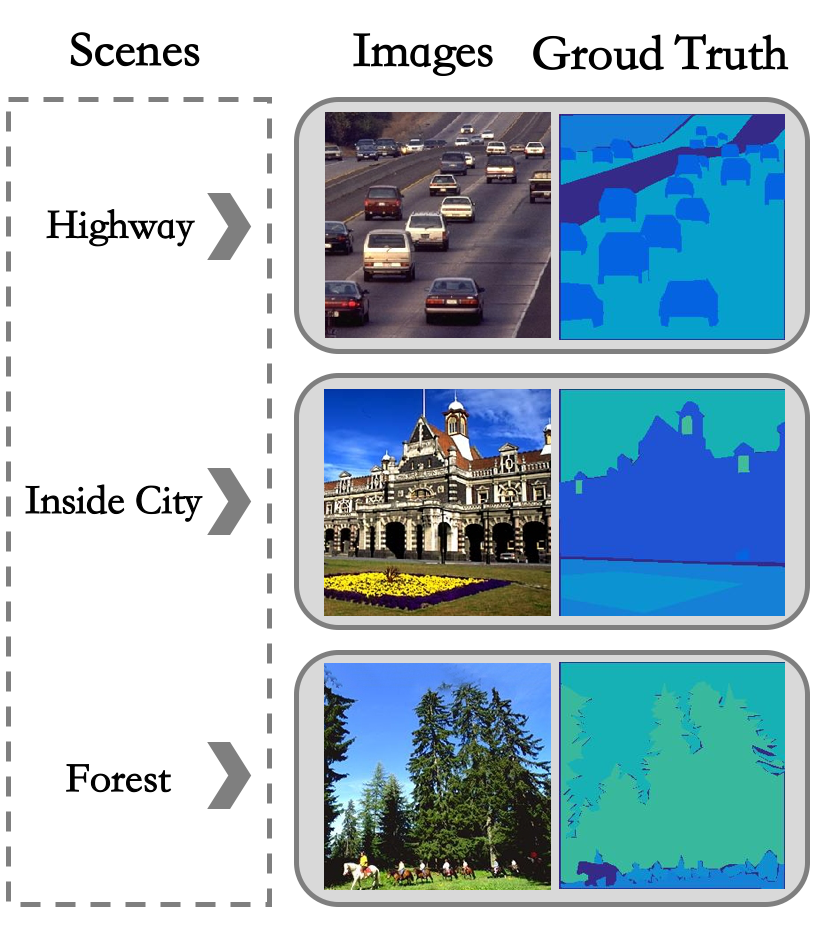
\includegraphics[width=0.95\columnwidth]{fig1.png}
\caption{Examples of semantic segmentation.}
\label{fig:example}
\end{figure} 


\noindent
  $\bullet$ A cascade segmentation network architecture to refine the final segmentation results.
  
\noindent
  $\bullet$ Incorporate the idea of hard mining into an attention module.
  
\noindent
  $\bullet$ Validate CasNet on both Sift Flow\upcite{6} and Stanford Background\upcite{7} datasets.


\section{Related Works}
\label{s:Related}
\noindent
Semantic segmentation aims to relate an unique semantic class (road, water, sea etc.) to each pixel of the input image. Both the global and local features have great impacts on the final performance of this task. Consequently, in terms of feature representations, the mainstream approaches can be divided into traditional hand-craft features and deep features based on deep neural networks. 

In recent years, traditional methods have obtained several solutions on image segmentation. Considering the context information, several methods rely on MRF, CRF or other types of graphical models to ensure consistency of labeling\upcite{8-10}. Besides, most methods employ pre-segmentation in order to produce super-pixels or segmented candidates, and extract features from these individual segments along with the combinations of adjacent segments.
\begin{figure*}[!ht]
\centering
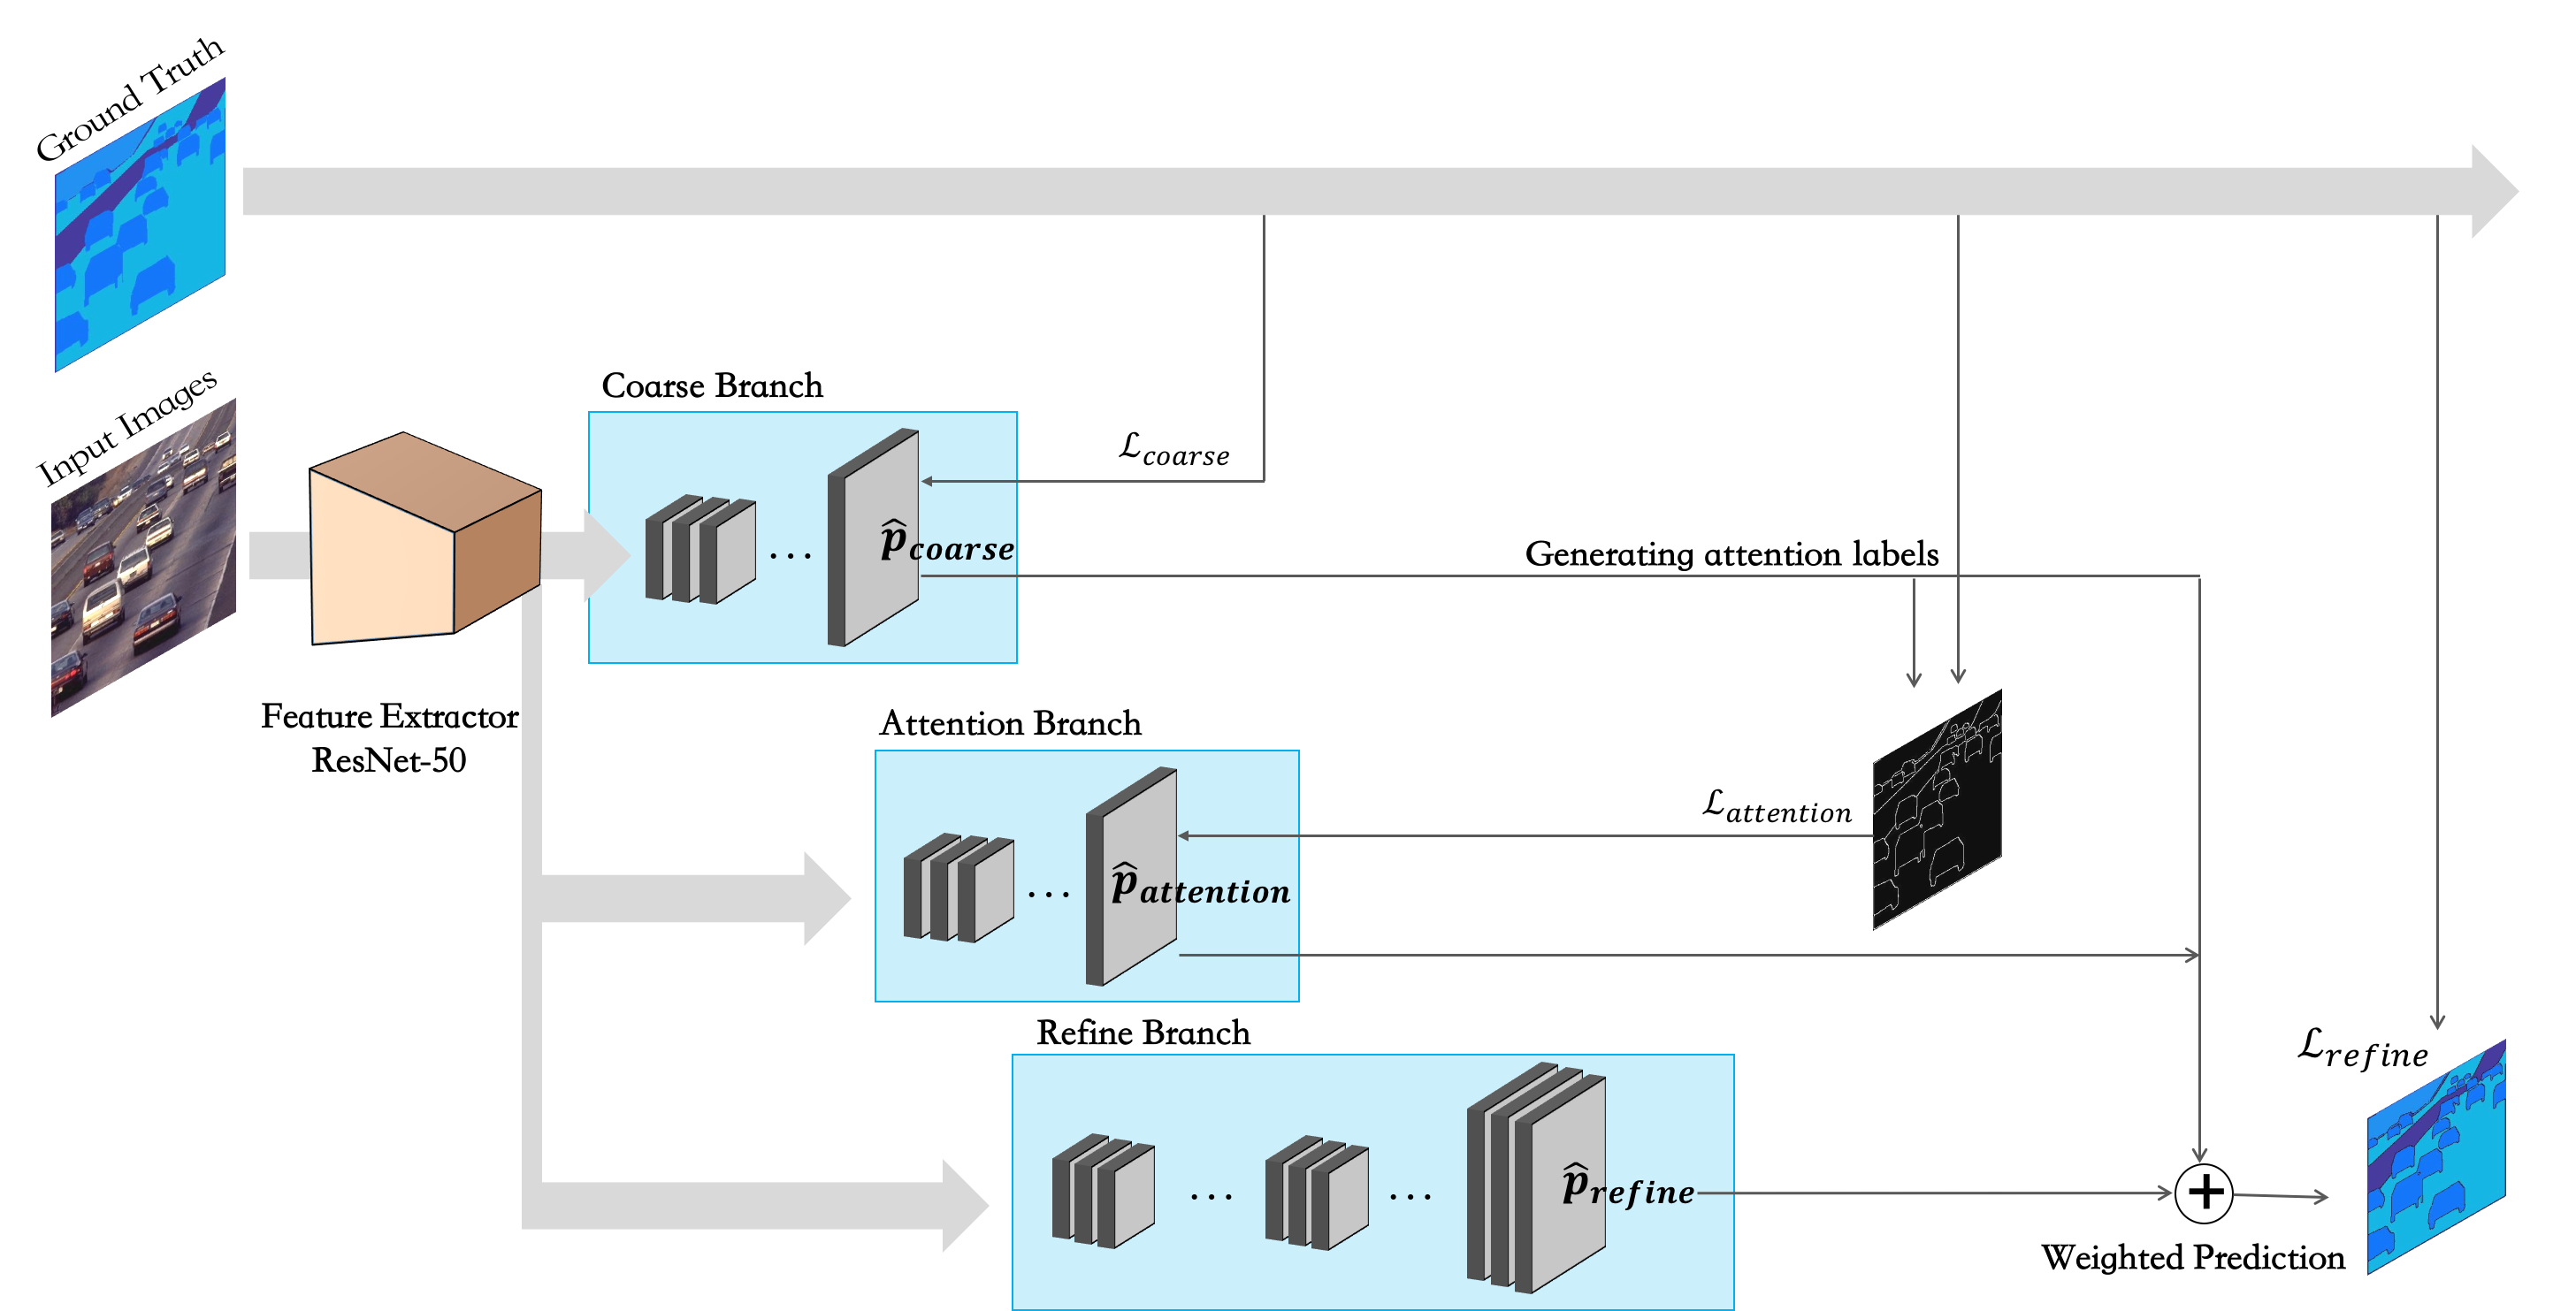
\includegraphics[width=1.9\columnwidth]{fig2.png}
\caption{A Cascade Coarse to Fine Network Architecture for Semantic Segmentation.}
\label{fig2}
\end{figure*} 

Meanwhile, the neural networks, particularly the CNNs that yield hierarchies of features have achieved great progress in  this pixel-level prediction task. \cite{11} is the first work that use CNNs for this semantic segmentation. They propose a multi-scale convolution neural network, which extracts the feature representations from different scales of local regions. The experimental results show that the network has capacities of learning texture, shape and domain information implicitly, and achieves better performance than traditional hand-craft features. In addition, the network is also able to generalized to the RGB-D images\upcite{12}. To ensure a good visual coherence and a high class accuracy, \cite{13} propose a method to capture long range (pixel) label dependencies in images. They use a recurrent architecture of CNNs to capture a long range label dependency while keeping a tight control over the capacity. The procedure is based on supervised deep learning strategies. \cite{14-16} train the parametric CNNs by sampling image patches, which speeds up the training time dramatically. However, they find that patch-based CNNs suffer from local ambiguity problems. \cite{14} estimate the global potential in a non-parametric framework and propose a large margin based CNN metric for better global potential estimation. \cite{15,16} introduce quaddirectional 2D Recurrent Neural Networks to model the long range dependencies among pixels which is able to embed the global image context into the compact local representation and significantly enhance their discriminative power.


	At the same time, researchers attempt to use the pre-trained CNNs for semantic segmentation. \cite{17} obtain the local and proximal features by using the ConvNet while distant and global features are produced from Alex-net\upcite{18}. These above features are further aggregated to predict the categories. Differ from these methods, \cite{19} present a fully convolutional network which is able to take input of arbitrary size and produce correspondingly-sized output with efficient inference and learning. They use the CNNs trained on ImageNet as a feature extractor and transfer their learned representations by fine-tuning on the task-specific datasets. \cite{20} propose deep networks by combining the responses at the final DCNN layer with a fully connected CRF. The fully connected pairwise CRF has an ability to capture fine edge details which boosts the final performance. In \cite{21}, it presents that the main problem of the current FCN-based models is lack of the incorprating  of context information. They exploit the capability of global context information by different-region-based context aggregation through a pyramid pooling module together with the proposed pyramid scene parsing network (PSPNet).



\section{Method}
\label{s:Method}
\noindent


Inspired by online hard example mining(OHEM) algorithm, we propose a cascade coarse to fine network architecture CasNet. The framework of the proposed CasNet is shown in Figure~\ref{fig2}. Given an image, firstly a ResNet is employed to extract feature representation. Then, the proposed CasNet will be exploited to learn the task-specific objective. In the following subsection, Section~\ref{s:feature} illustrates how to apply a ImageNet pre-trained model to extract feature representation of the given image. At last, Section~\ref{s:casnet} provides the detailed information of the cascade coarse to fine semantic segmentation network, particularly the three branches which are expected to collaboratively learn to predict from coarse to fine.


\subsection{Feature Extraction Network}
\label{s:feature}
\noindent

We choose ResNet-50 which is pre-trained on ImageNet as our feature extractor. ResNet originally is designed for image classification which won ILSRVC 2015 competition and surpass the human performance on ImageNet dataset. It has super capacities of extracting hierarchical representations. Considering the computation resources and memory consumption, we choose ResNet-50 rather than ResNet-101, but it can still achieve comparable accuracy. In Figure~\ref{fig2}, the hexahedron presents the feature extractor. Although we just use this simplified figure to present the ResNet-50, it is composed by five stages with different configurations of layers and a classification stage. The building block of ResNet can be defined as:

\begin{equation}\label{equ1}
\setlength\abovedisplayskip{4pt}
\setlength\belowdisplayskip{4pt}
\begin{split}
y = F(x, \{W_{i}\}) + x \\
\end{split}
\end{equation} 
where $x$ and $y$ denote the input and output of a layer. The function $F(x, \{W_{i}\})$ indicates the residual mapping while the $W_{i}$ represents a group of learnable weights. The operation $F + x$ is performed by a shortcut connection and element-wise which in fact combine the features of multi-scale. It benefits the segmentation task a lot. For semantic segmentation,  the context is important to predict the correct label of each pixel instance. But it is difficult to determine the context boundary of each pixel, since different objects may have different contours. The problem becomes more complicated when considering the various perspective of each images. A simple yet effective method to solve this problem is to integrate multi-scale features for label predicting. Consequently, the residual error model itself has the property of extracting and integrating multi-scale features, which can be seen from Equation \ref {equ1}. From the unravelled view by Veit et al.~\upcite{22}, a two-unit ResNet is equivalent to an ensemble of four sub-networks with different receptive fields. So the whole ResNet-50 can be expanded as a linearly growing ensemble of sub-networks, which can extract and integrate multi-scale features.

Besides, there are two improvements adopted by ResNet-50 to make it more suitable for semantic segmentation. First, we only keep the first three pooling layers in order to preserve the resolution. So the final resolution of the prediction is 1/8 of the original input image. Secondly, we replace the convolutional layer in the last two stages with the dilated convolutions. It can help to enlarge the reception field of predicted feature maps.



\subsection{A Cascade Coarse to Fine Architecture}
\label{s:casnet}
\noindent

The architecture of CasNet is shown as Figure~\ref{fig2}. There are three horizontal lines running from input to the target. They are the proposed cascade branches: a coarse segmentation branch as a baseline result, an attention branch to predict the difficulty of labelling each pixel instance, and a refine segmentation branch to refine the final segmentation results. 
These three branches share a common feature extraction network while focus on their own targets.

\subsubsection{The Coarse Segmentation Branch}
\label{s:cbb}
\noindent

The coarse segmentation branch is a baseline model for semantic segmentation which is on the first row in Figure~\ref{fig2}. We adopt a FCN that consisted of two convolutional layers to predict the semantic classes for relatively easy and confident regions. Since the resolution is 1/8 of the original input image, the feature maps are up-sampled by bilinear interpolation. Finally, a pixel-wise softmax loss is adopted to predict the probabilities of each pixel. We first formulate the coarse segmentation branch which produces the probability map as Equation \ref{equ2}, and the loss function is also defined as Equation \ref{equ3}: 
\begin{equation}\label{equ2}
\setlength\abovedisplayskip{8pt}
\setlength\belowdisplayskip{8pt}
\begin{split}
p_{c}(i,j) &= \mathcal{F}_{coarse}(x, \mathcal{W}_c)\\
\end{split}
\end{equation} 
\begin{equation}\label{equ3}
\setlength\abovedisplayskip{8pt}
\setlength\belowdisplayskip{8pt}
\begin{split}
\mathcal{L}_{coarse}(y, p_c) &= - \frac{1}{N}[\sum_{(i,j)\in I}\log(p^{y(i,j)}_c(i,j))]\\
\end{split}
\end{equation} 
where $(i,j)$ is the pixel's location of the given image and $x$ is the input features extracted by feature extraction network in Section~\ref{s:feature}. $ \mathcal{F}_{coarse}$ represents the coarse segmentation branch with the trainable weights $ \mathcal{W}_c$. And the $p_{c}(i,j)$ denotes the computed probability of each pixel. Particularly, the $p_{c}(i,j)$ in Equation \ref{equ2} is a $K$ dimensional vector (whose elements sum to 1) that represents the estimated probability of the class label taking on each of the $K$ different possible values while the $p^{y(i,j)}_c(i,j)$ in Euation \ref{equ3} is account for the estimated probability of ground truth category $y(i,j)$. So the  Equation \ref{equ3} shows the standard $softmax$ loss which accumulates the loss of each pixels and then is averaged by the number of pixels $N$. 

Equation \ref{equ2} and \ref{equ3} allow to train the coarse segmentation branch and produce the coarse prediction results that are useful for the following two branches.


\subsubsection{The Attention Branch}
\label{s:ab}
\noindent

After the first stage of segmentation, there still exists several regions which cannot be determined by the coarse segmentation network. To our knowledge, each segmentation image contain a large number of easy pixel instances and a small number of difficulty pixel instances. Paying more attention on these difficulty pixel instances can make the training process converge faster and efficiently. However, we have no labels that indicate which regions are difficult. 

From previous research work, hard example mining is one of the commonly used training techniques for machine learning. The traditional implementation is a continuous iterative process which could be divided into two steps. Firstly, the training model is fixed to figure out the difficult examples, and the training set is updated by adding a certain rate of difficult examples. Secondly, with the updated training set, the model is re-trained.

In this paper, the two-step process of hard example mining is improved to an end-to-end learning framework. For semantic segmentation, each pixel should be assigned a category label. So a single image contain enough training samples for hard example mining. The attention branch is used to predict the segmentation difficulty of each pixel in terms of the results of coarse segmentation branch. It shares the same feature extraction network as the coarse segmentation branch. Moreover, they even have the similar network structure.  As shown in Equation \ref{equ4}, the $\mathcal{F}_{attention}$ is the attention branch with the learnable weights $ \mathcal{W}_a$ and the input is also $x$, which is the shared feature as Equation \ref{equ2}. The major difference is that the attention branch is a two-category semantic segmentation network while the coarse branch is responsible for learning much more categories.
\begin{equation}\label{equ4}
\setlength\abovedisplayskip{8pt}
\setlength\belowdisplayskip{8pt}
\begin{split}
p_{a}(i,j) &= \mathcal{F}_{attention}(x, \mathcal{W}_a)\\
\end{split}
\end{equation} 

During the training process, the attention branch is supervised by a label map with 0/1 values, indicating  easy or difficult for the pixel in corresponding position. The attention branch is cascaded behind the coarse segmentation branch, so the label map $\hat{y}$ can be generated by a comparison between the prediction of the coarse segmentation branch $p_{c}^k(i,j)$ and the segmentation ground truth $y(i,j)$. 0 indicates the pixel is misclassified by the coarse segmentation branch, while 1 represents a correct prediction. The 0/1 label map is used as the ground truth of the attention branch in Equation \ref{equ6}, supervising the attention branch to learn the segmentation difficulty of each pixel.
\begin{equation}\label{equ5}
\setlength\abovedisplayskip{8pt}
\setlength\belowdisplayskip{8pt}
\begin{split}
\hat{y}(i,j) = 
\begin{cases}
1, &\arg\underset{k \in \mathcal{K}}{\max}\,p_{c}^k(i,j)=y(i,j)\\
0, &otherwise
\end{cases}
\end{split}
\end{equation} 
\begin{equation}\label{equ6}
\setlength\abovedisplayskip{8pt}
\setlength\belowdisplayskip{8pt}
\begin{split}
\mathcal{L}_{attention}(\hat{y}, p_a) = - \frac{1}{N}[\sum_{(i,j)\in I}log(p^{\hat{y}(i,j)}_a(i,j))]\\
\end{split}
\end{equation}
where $\hat{y}$ is the pixel-wise binary label. $\arg\underset{k \in \mathcal{K}}{\max}\,p_{c}^k(i,j)$ denotes the category which holds the maximum estimated probability among all the categories $\mathcal{K}$. If this category is equal to the ground truth, positive value $1$ will be assigned to $\hat{y}$, indicating that this pixel is correctly predicted by coarse segmentation branch. Otherwise, $0$ will be the new label of this pixel that represents it is difficult for coarse branch.

During the testing process, the attention branch heuristically filter out the hard examples online.

%The attention branch is proposed to learn a soft-attention, which is a one-channel feature map with the same resolution as the input image. It is mainly used to indicate the segment difficulty of each pixel. The idea behind is simple yet effective. 


%It makes the end-to-end learning possible by heuristically filtering out the hard examples online. The final segmentation results relay more on the coarse segmentation branch if the pixel is predicted as an easy one. Otherwise, the fine segmentation network takes up a larger proportion. Inspired by online hard example mining, the attention branch with a heuristic strategy is introduced to CasNet to predict the difficult of each pixel. And the final segmentation results are promoted by hard sample selection.


\subsubsection{The Refine Segmentation Branch}
\label{s:rsb}
\noindent

The refine segmentation branch is cascaded behind the coarse and the attention as shown on the third row in Figure~\ref{fig2}. This branch is more complicated compared with the first two branches. It contains a fine segmentation network and a weighted summation of unit to refine the final segmentation results.

Since the coarse segmentation branch is hard to segment all the pixels correctly, the pixel which can be segment correctly by the coarse segmentation branch is denote as easy pixel instances, while the others are difficult ones.
A fine segmentation network is introduced to focus on reclassification of the difficult pixel instances. Inspired by the PSPNet~\upcite{21}, pyramid pooling is adopted by the fine segmentation network to extract multi-scale features. And the final segmentation results is a weighted summation of the coarse segmentation branch and the fine segmentation network, with the weighting coefficient predicted by the attention branch. The final segmentation results relay more on the coarse segmentation branch if the pixel is predicted as an easy one. Otherwise, the fine segmentation network takes up a larger proportion. 

The three branches are cascaded one by one, and constitute an end-to-end learning network with multiple loss functions.
\begin{equation}\label{equ7}
\setlength\abovedisplayskip{8pt}
\setlength\belowdisplayskip{8pt}
\begin{split}
p_{f}(i,j) = \mathcal{F}_{fine}(I, \mathcal{W}_f)\\
\end{split}
\end{equation}
\begin{equation}\label{equ8}
\setlength\abovedisplayskip{8pt}
\setlength\belowdisplayskip{8pt}
\begin{split}
p_{refine}(i,j) &= p_{a}(i,j) \cdot p_{c}(i,j)\\
&+ (1-p_{a}(i,j)) \cdot p_{f}(i,j)\\
\end{split}
\end{equation}
\begin{equation}\label{equ9}
\setlength\abovedisplayskip{8pt}
\setlength\belowdisplayskip{8pt}
\begin{split}
\mathcal{L}_{refine}(y, p_{refine}) = - \frac{1}{N}[\sum_{(i,j)\in I}log(p^{y(i,j)}_{refine}(i,j))]\\
\end{split}
\end{equation}

Finally, 6 loss functions are
computed on {A(1)
, . . . , A(6)} using the Equation 1 to provide
deep supervision to this network.


\begin{figure*}[ht]
\centering
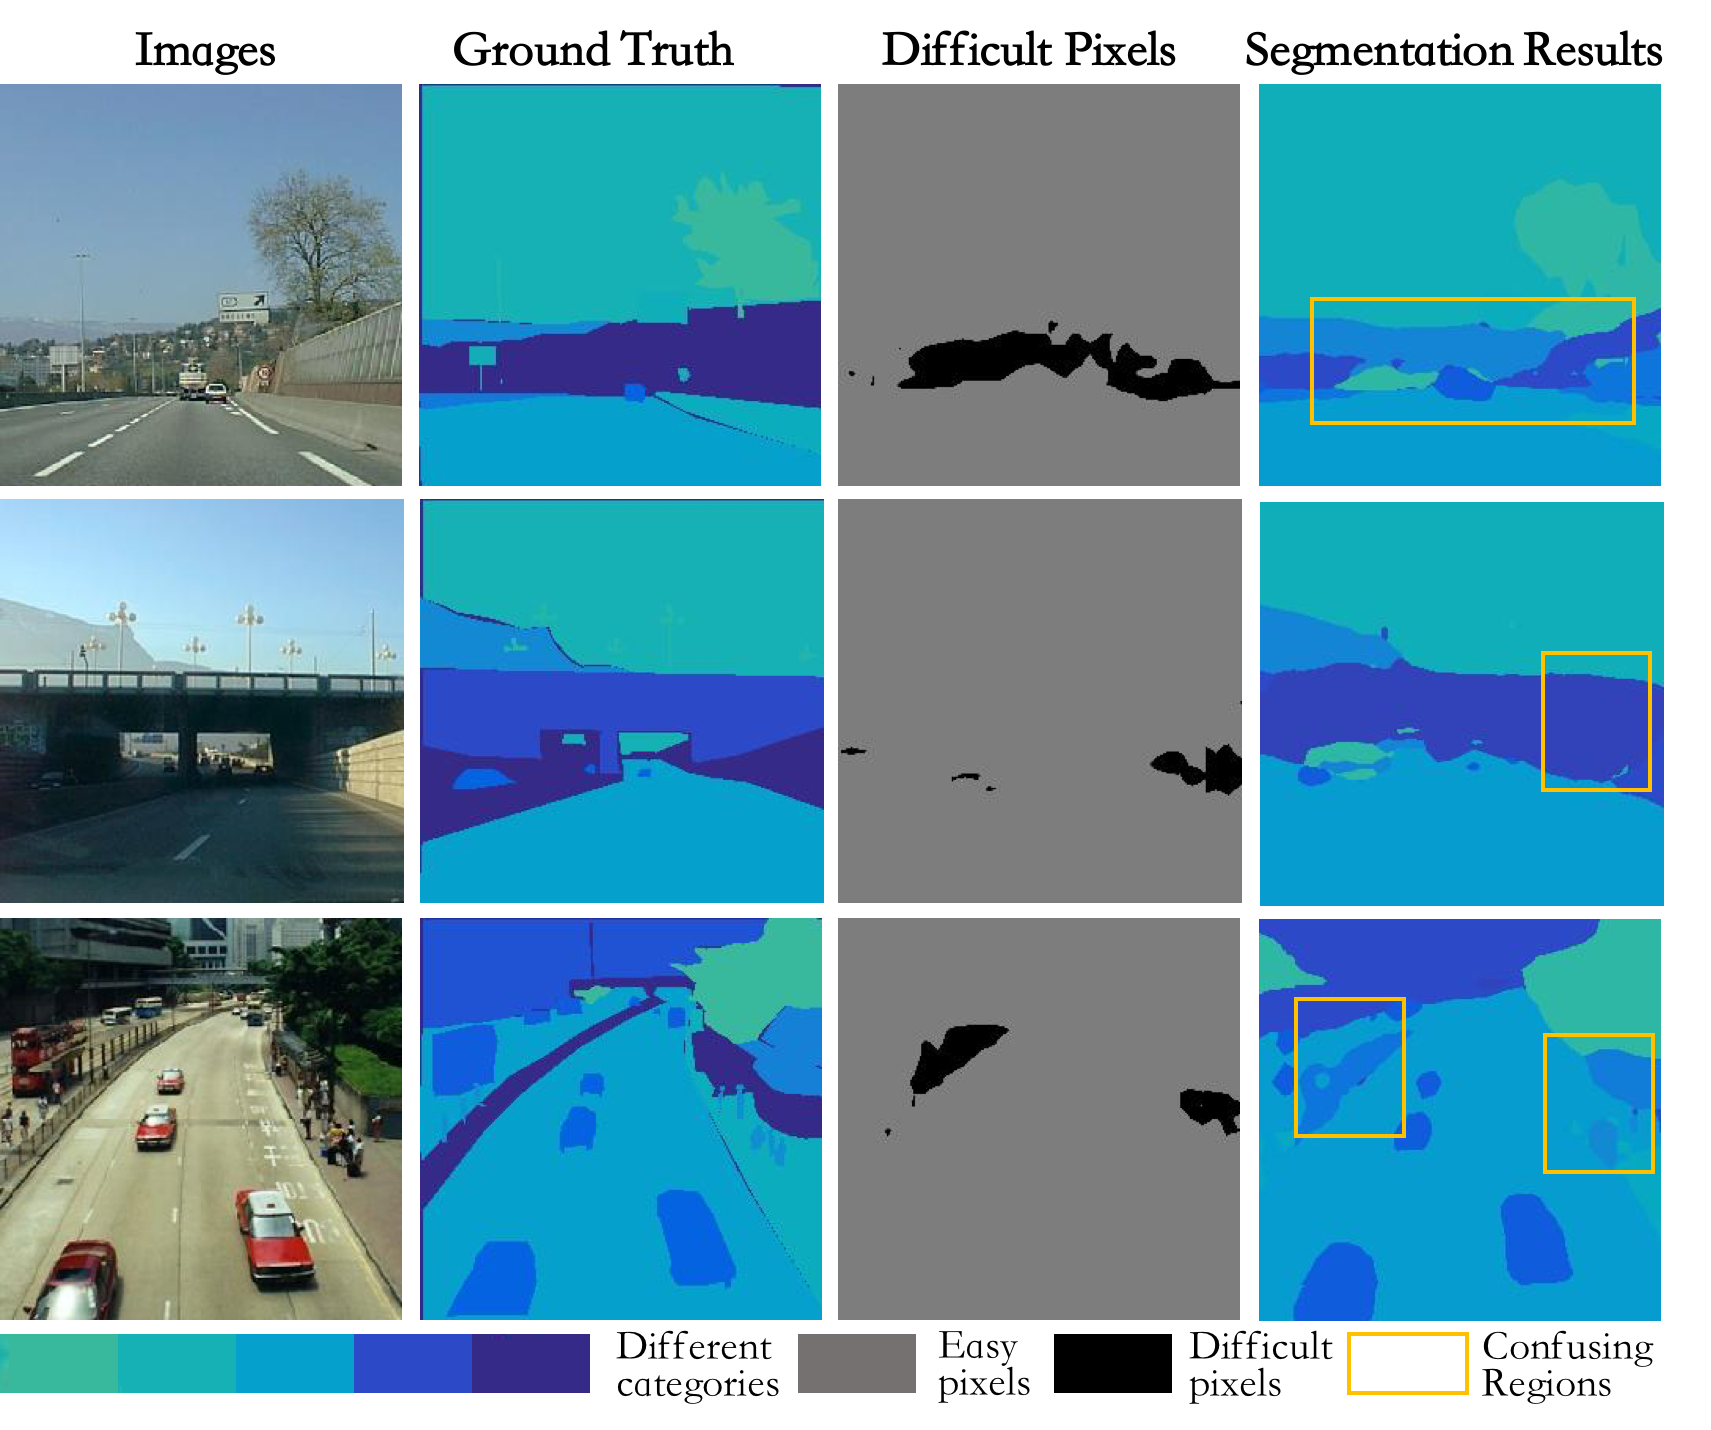
\includegraphics[width=1.9\columnwidth]{fig3.png}
\caption{The visualization predicting result of CasNet.}
\label{fig3}
\end{figure*} 

\section{Experimental results}
\label{s:results}
\noindent
In this subsection, we present the detailed information about the implementation of CasNet. Moreover, we compare our model to the current state-of-the-art methods and this proposed model achieves superior performances among the existing methods.

\subsection{Datasets}
\noindent
We prove the effectiveness of CasNet on two semantic segmentation datasets, which are SIFT Flow and Stanford Background, respectively. The SIFT Flow dataset contains 2688 samples each has 256x256 pixels with RGB channels. 2488 images are used as a training set while the rest 200 images are used for testing. The dataset defines a total of 33 semantic categories, but the distribution of category is nonuniform.

The Stanford Background dataset contains 715 images with different image sizes, but no more than 320x240 pixels. According to the previous research and testing methods, this paper divides the dataset by 5x cross validation method, and 572 images are used as training samples while 143 samples as the test samples. The Stanford Background dataset contains eight semantic categories, and the category distribution is more balanced than the SIFT Flow dataset.


\subsection{Network Configuration}
\noindent
The implementation of our CasNet is based on public platform Caffe~\upcite{23}. The training procedure uses stochastic gradient descent (SGD) algorithm via end-to-end learning. Our model adopt pre-trained models like most related work~\cite{21} on semantic segmentation. The learning rate is initially set to 1e-4 and then decreased by a factor of 10 when the validation set accuracy stopped improving. In total, the learning rate is repeatedly decreased 2 times. The momentum and weight decay are set to 0.9 and 0.0001.

Data argumentation is widely applied to semantic segmentation in order to avoid overfit. Various kinds of transformations are used to expand the training sizes so as to improve the generalisation of the proposed networks. In our experiments, we also employ this kind of methods by expanding the input images 1-2 times and randomly cropping 233x233  area for training.  Larger input size and mini-batch can help improve the segmentation performance. Due to the limitation of both computation and memory, we only use 233*233 images and the mini-batch is 4.



\subsection{Comparison Results}
\noindent

During the comparison, we first conduct several experiments on SIFT Flow dataset.
Firstly, we compare CasNet with a baseline model, which is composed by a ResNet and two FCN layers. The baseline model is a  typical FCN segmentation network based on ResNet-50, and has a same network architecture as the coarse branch of CasNet. The comparison result is show as Table~\ref{t:self1}, CasNet leads to about 1\% gain in comparison to the baseline ResNet segmentation network. Since cascade coarse to fine network architecture is effective for refining the segmentation results.

\begin{table}[h]
\large
\setlength{\belowcaptionskip}{12pt}
\caption{The Comparison Result with Baseline Model on SIFT Flow.}
\label{t:self1}
\centering
\begin{tabular}{ccc}
\hline 
Methods & Pixel acc. \\
\hline
Baseline(ResNet) & 90.52 \\
CasNet & 91.6  \\
\hline
\end{tabular}
\end{table}

A visualisation of the intermediate network feature is show in Figure~\ref{fig3}, which consists of four columns. The first column presents the input images and second column shows the ground truth labels. In particular, the third column indicates hard pixels predicted by the attention branch of CasNet while the last column is the segmentation results of the network. As can be seen from the third and fourth columns of Figure~\ref{fig3}, the CasNet can indeed predict the hard pixel samples which are indicated in the yellow square box of last column in Figure~\ref{fig3}.

In addition, on the SIFT Flow dataset, we compare the CasNet to other segmentation methods. Pixel-level semantic segmentation is usually measured by two accuracy measures: Pixel Accuracy and Class Accuracy. The average pixel accuracy is the percentage of the total number of pixels that correctly classified on the test set, and it is usually measured by the intersection-over-union (IoU). The average category accuracy is the average of the correct rate for each category of pixel classification. The experimental results which is shown in Table \ref{table1} which prove that CasNet achieves an accuracy of 91.6\%, and outperform the current state-of-the-art results.

\begin{table}[h]
\large
\setlength{\belowcaptionskip}{12pt}
\caption{The Segmentation Results on SIFT Flow.}
\label{table1}
\centering
\begin{tabular}{ccc}
\hline 
Methods & Pixel acc. & Class acc. \\
\hline
Liu et al.\upcite{6} & 76.7 & - \\
Tighe et al. SVM\upcite{25} & 75.6 & 41.4 \\
Tighe et al. SVM+MRF\upcite{26} & 78.6 & 39.2 \\
Farabet et al. natural\upcite{11} & 72.3 & 50.8 \\
Farabet et al. balanced\upcite{11} & 78.5 & 29.6 \\
Pinheiro et al.\upcite{13} & 77.7 & 29.8 \\
Liang et al. RCNN\upcite{24} & 84.3 & 41.0 \\
Shelhamer et al. FCN-8s\upcite{4} & 85.9 & 53.9 \\
\textbf{CasNet} & 91.6 & 52.5 \\

\hline
\end{tabular}
\end{table}

In order to prove the generalisation of the learning scheme of the semantic segmentation, we test the CasNet on another dataset called Stanford Background by using the same architecture and configurations. Table \ref{table2} shows that on the Stanford Background dataset, CasNet achieved 89.7\% pixel average accuracy and 75.4\% classification accuracy. Some of the prediction results are shown in Figure~\ref{fig4}, which can be clearly seen the predicted results.

\begin{table}[h]
\large
\setlength{\belowcaptionskip}{12pt}
\caption{The Segmentation Results on Stanford background.}
\label{table2}
\centering
\begin{tabular}{ccc}
\hline 
Methods & Pixel acc. & Class acc. \\
\hline
Gould et al.\upcite{7} & 76.4 & - \\
Tighe and Lazebnik\upcite{25} & 77.5 & - \\
%Socher et al.\upcite{27} & 78.1 & - \\
Eigen and Fergus\upcite{28} & 75.3 & 66.5 \\
Singh and Kosecka\upcite{27} & 74.1 & 62.2 \\
Lempitsky et al.\upcite{10} & 81.9 & 72.4 \\
Liang et al. RCNN\upcite{24} & 83.1 & 74.8 \\
\textbf{CasNet} & 89.7 & 75.4 \\
\hline
\end{tabular}
\end{table}

\begin{figure}[ht]
\centering
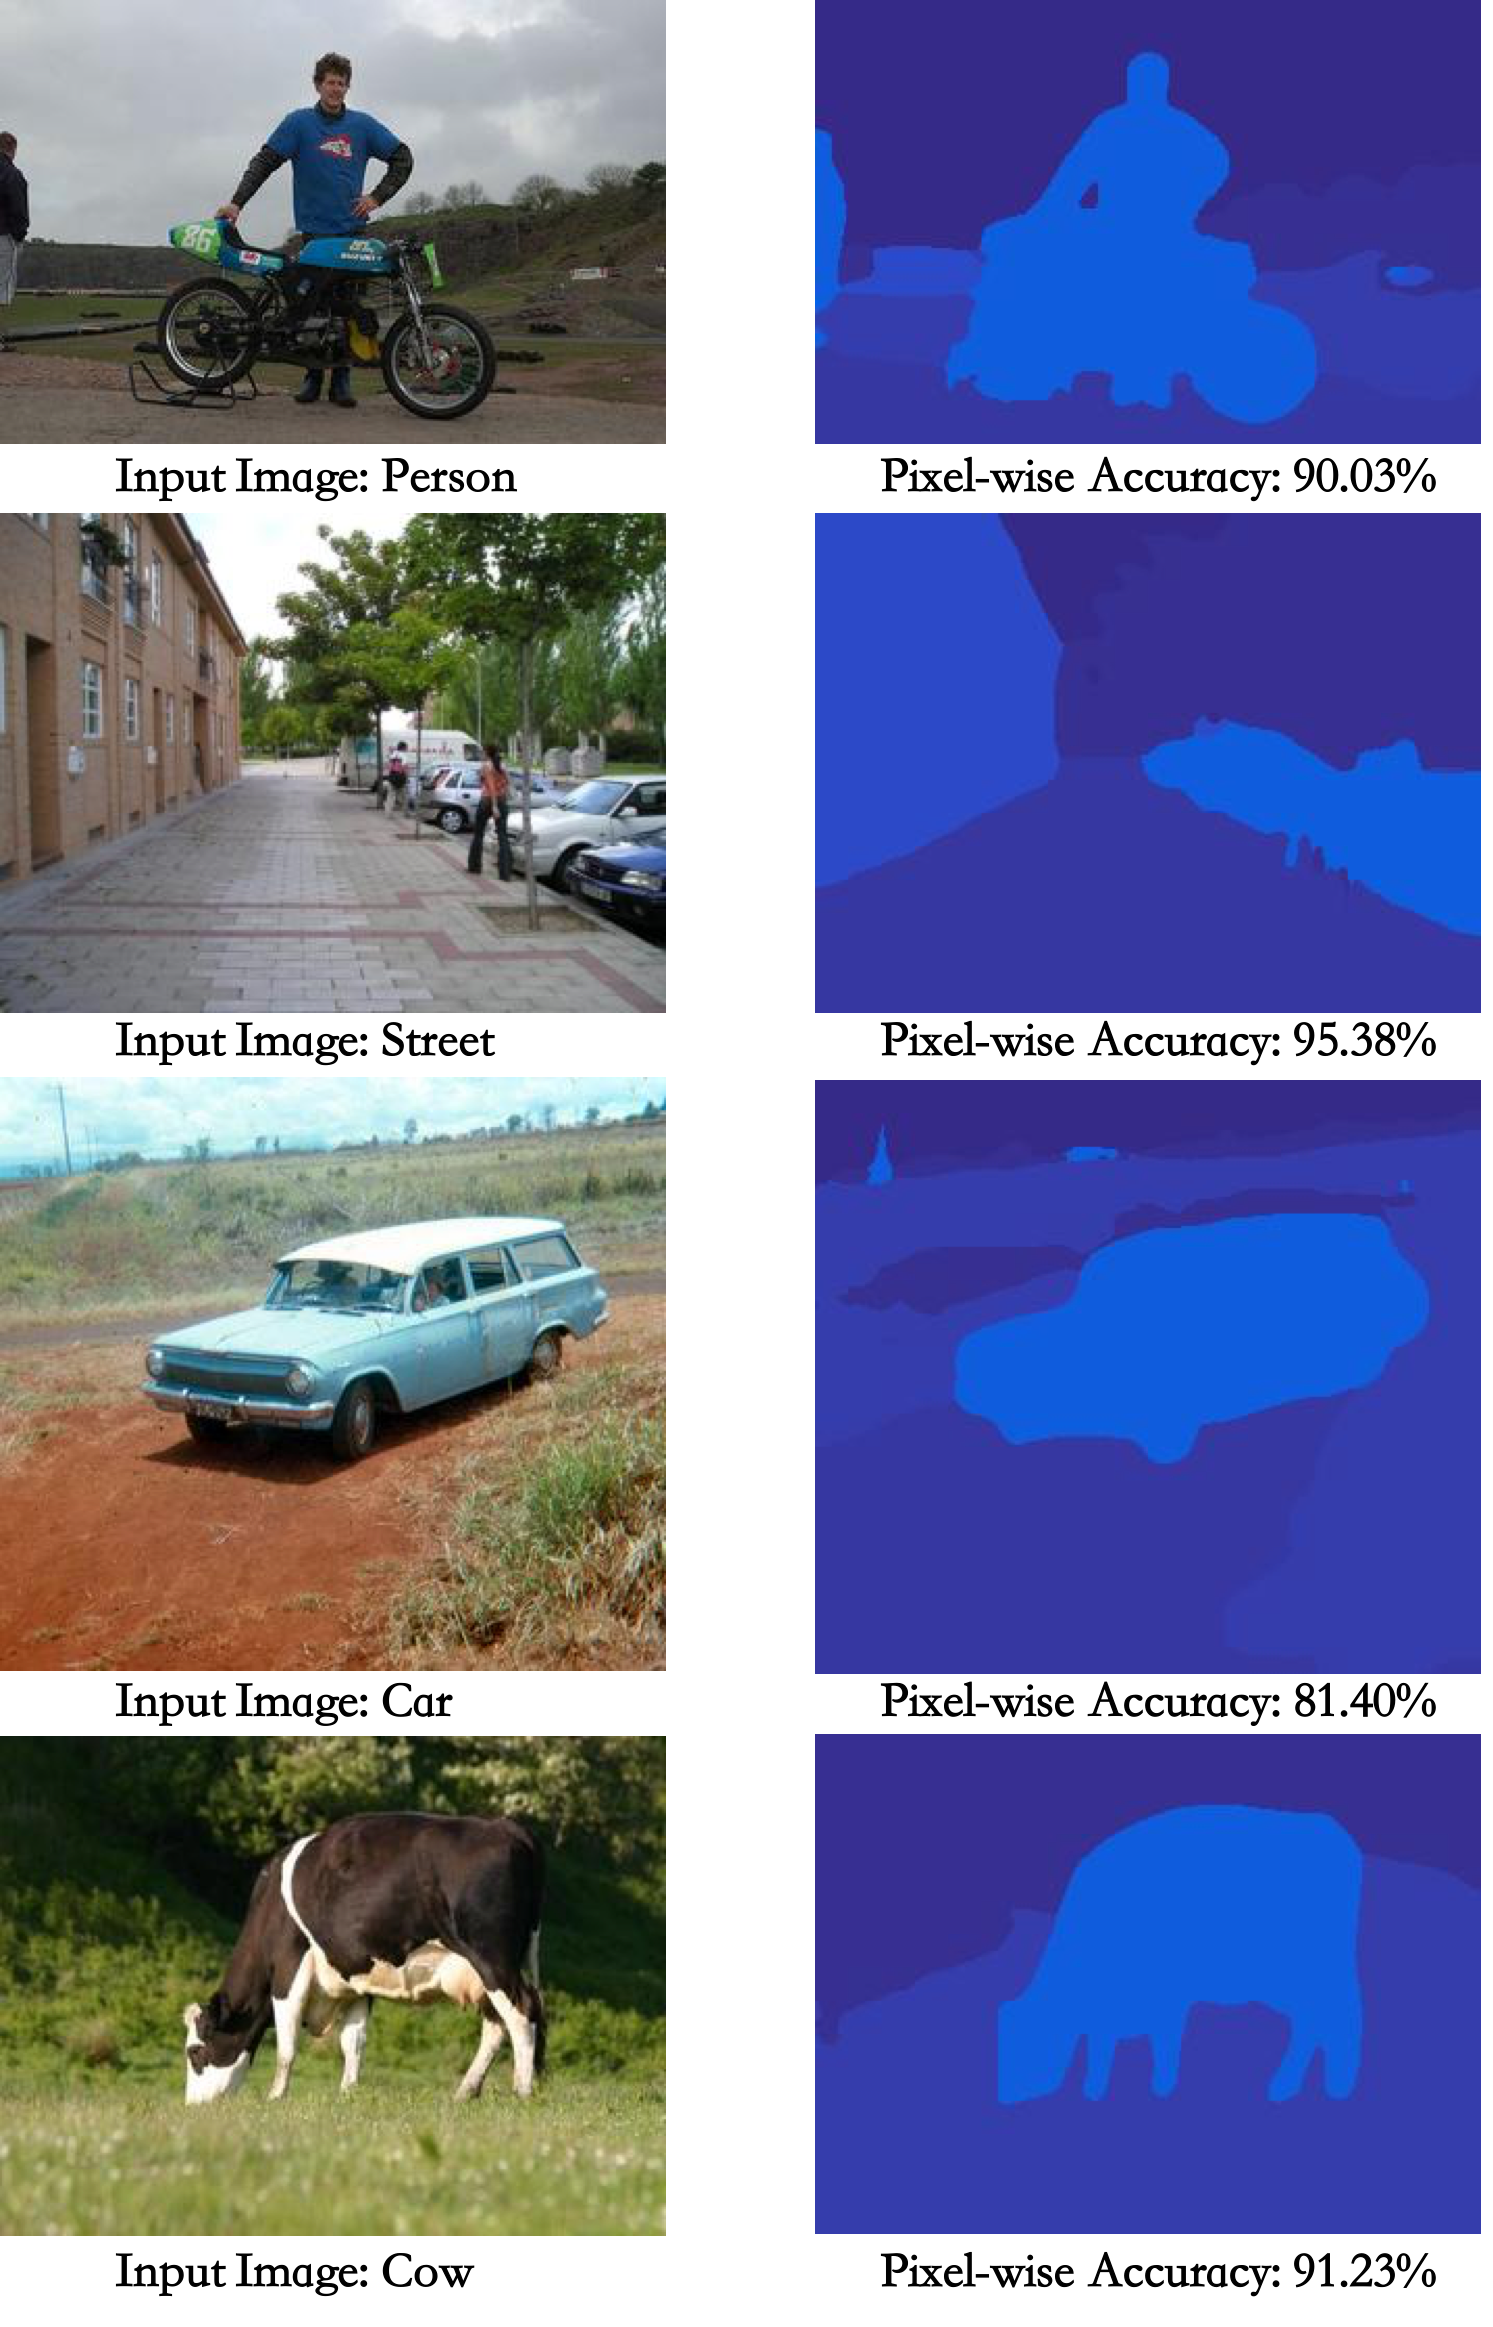
\includegraphics[width=0.85\columnwidth]{fig4.png}
\caption{The predict results on Stanford Background dataset.}
\label{fig4}
\end{figure} 

\section{Conclusions}
\noindent

Inspired by the idea of hard mining, we propose a novel cascade coarse to fine segmentation network architecture.
This network include three branches, in which the first is a coarse segmentation network.
While the second branch is an attention network used to predict the difficulty of segmenting each pixel.
And the third branch refines the final segmentation results by taking a weighted average of multiple branches.
In order to evaluate the performance of CasNet, we conduct experiments on two public datasets including Sift Flow Dataset and Stanford Background Dataset. 
We show how to train these three branches in an end-to-end manner. And finally, the experimental results show that compared to all existing models, our CasNet consistently yields the best performance, with the accuracy of 91.6\% and 89.7\%, respectively.


\vskip 2mm
\zihao{5}
\noindent
\textbf{Acknowledgements}
\vskip 2mm

\zihao{5--}
\noindent
This work was supported in part by the National Science Foundation of China (NSFC) under Grant Nos. 91420106, 90820305, and 60775040, and by the National High-Tech R\&D Program of China under Grant No. 2012AA041402.

\vskip 2mm
\zihao{5}
\noindent
\textbf{\zihao{5}References}
\vskip 2mm


\begin{thebibliography}{99}
\zihao{5-} \addtolength{\itemsep}{-1em}
\vspace {1.5mm}

%\bibitem[1]{1}
%Krizhevsky A, Sutskever I, Hinton G E. Imagenet classification with deep convolutional neural networks[C]//Advances in neural information processing systems. 2012: 1097-1105.

%\bibitem[4]{4}
%Graves A, Mohamed A, Hinton G. Speech recognition with deep recurrent neural networks[C]//Acoustics, speech and signal processing (icassp), 2013 ieee international conference on. IEEE, 2013: 6645-6649.
%
%\bibitem[5]{5}
%Sermanet P, Eigen D, Zhang X, et al. Overfeat: Integrated recognition, localization and detection using convolutional networks[J]. arXiv preprint arXiv:1312.6229, 2013.
%
%\bibitem[6]{6}
%Ioffe S, Szegedy C. Batch normalization: Accelerating deep network training by reducing internal covariate shift[J]. arXiv preprint arXiv:1502.03167, 2015.
%
%\bibitem[7]{7}
%He K, Zhang X, Ren S, et al. Deep residual learning for image recognition[C]//Proceedings of the IEEE Conference on Computer Vision and Pattern Recognition. 2016: 770-778.

%\bibitem[8]{8}
%Liu C, Yuen J, Torralba A. Sift flow: Dense correspondence across scenes and its applications[J]. IEEE transactions on pattern analysis and machine intelligence, 2011, 33(5): 978-994.
%
%\bibitem[9]{9}
%Gould S, Fulton R, Koller D. Decomposing a scene into geometric and semantically consistent regions[C]//Computer Vision, 2009 IEEE 12th International Conference on. IEEE, 2009: 1-8.
%
%
%\bibitem[10]{10}
%Russell C, Kohli P, Torr P H S. Associative hierarchical crfs for object class image segmentation[C]//Computer Vision, 2009 IEEE 12th International Conference on. IEEE, 2009: 739-746.
%
%\bibitem[11]{11}
%Kumar M P, Koller D. Efficiently selecting regions for scene understanding[C]//Computer Vision and Pattern Recognition (CVPR), 2010 IEEE Conference on. IEEE, 2010: 3217-3224.
%
%\bibitem[12]{12}
%Lempitsky V, Vedaldi A, Zisserman A. Pylon model for semantic segmentation[C]//Advances in neural information processing systems. 2011: 1485-1493.
%
%\bibitem[13]{13}
%Farabet C, Couprie C, Najman L, et al. Learning hierarchical features for scene labeling[J]. IEEE transactions on pattern analysis and machine intelligence, 2013, 35(8): 1915-1929.
%
%\bibitem[14]{14}
%Couprie C, Farabet C, Najman L, et al. Indoor semantic segmentation using depth information[J]. arXiv preprint arXiv:1301.3572, 2013.
%
%\bibitem[15]{15}
%Pinheiro P H O, Collobert R. Recurrent Convolutional Neural Networks for Scene Labeling[C]//ICML. 2014: 82-90.
%
%\bibitem[16]{16}
%Shuai B, Wang G, Zuo Z, et al. Integrating parametric and non-parametric models for scene labeling[C]//Proceedings of the IEEE Conference on Computer Vision and Pattern Recognition. 2015: 4249-4258.
%
%\bibitem[17]{17}
%Shuai B, Zuo Z, Wang G. Quaddirectional 2d-recurrent neural networks for image labeling[J]. IEEE Signal Processing Letters, 2015, 22(11): 1990-1994.
%
%\bibitem[18]{18}
%Shuai B, Zuo Z, Wang B, et al. Dag-recurrent neural networks for scene labeling[C]//Proceedings of the IEEE Conference on Computer Vision and Pattern Recognition. 2016: 3620-3629.
%
%\bibitem[19]{19}
%Mostajabi M, Yadollahpour P, Shakhnarovich G. Feedforward semantic segmentation with zoom-out features[C]//Proceedings of the IEEE Conference on Computer Vision and Pattern Recognition. 2015: 3376-3385.
%
%\bibitem[20]{20}
%Krizhevsky A, Sutskever I, Hinton G E. Imagenet classification with deep convolutional neural networks[C]//Advances in neural information processing systems. 2012: 1097-1105.
%
%\bibitem[21]{21}
%Long J, Shelhamer E, Darrell T. Fully convolutional networks for semantic segmentation[C]//Proceedings of the IEEE Conference on Computer Vision and Pattern Recognition. 2015: 3431-3440.
%
%\bibitem[22]{22}
%Chen L C, Papandreou G, Kokkinos I, et al. Semantic image segmentation with deep convolutional nets and fully connected crfs[J]. arXiv preprint arXiv:1412.7062, 2014.
%
%\bibitem[23]{23}
%Zhao H, Shi J, Qi X, et al. Pyramid Scene Parsing Network[C]//Proceedings of the IEEE Conference on Computer Vision and Pattern Recognition. 2017.
%
%\bibitem[24]{24}
%Jia Y, Shelhamer E, Donahue J, et al. Caffe: Convolutional architecture for fast feature embedding[C]//Proceedings of the 22nd ACM international conference on Multimedia. ACM, 2014: 675-678.
%
%\bibitem[25]{25}
%Tighe J, Lazebnik S. Superparsing: scalable nonparametric image parsing with superpixels[C]//European conference on computer vision. Springer Berlin Heidelberg, 2010: 352-365.
%
%\bibitem[26]{26}
%Tighe J, Lazebnik S. Finding things: Image parsing with regions and per-exemplar detectors[C]//Proceedings of the IEEE conference on computer vision and pattern recognition. 2013: 3001-3008.
%
%\bibitem[27]{27}
%Socher R, Lin C C, Manning C, et al. Parsing natural scenes and natural language with recursive neural networks[C]//Proceedings of the 28th international conference on machine learning (ICML-11). 2011: 129-136.
%
%\bibitem[28]{28}
%Eigen D, Fergus R. Nonparametric image parsing using adaptive neighbor sets[C]//Computer vision and pattern recognition (CVPR), 2012 IEEE Conference on. IEEE, 2012: 2799-2806.
%
%\bibitem[29]{29}
%Singh G, Kosecka J. Nonparametric scene parsing with adaptive feature relevance and semantic context[C]//Proceedings of the IEEE Conference on Computer Vision and Pattern Recognition. 2013: 3151-3157.
%
%\bibitem[30]{30}
%Liang M, Hu X. Recurrent convolutional neural network for object recognition[C]//Proceedings of the IEEE Conference on Computer Vision and Pattern Recognition. 2015: 3367-3375.
%
%\bibitem[31]{31}
%Sung, K-K., and Tomaso Poggio. "Example-based learning for view-based human face detection." IEEE Transactions on pattern analysis and machine intelligence 20.1 (1998): 39-51.
%
%\bibitem[32]{32}
%Veit, Andreas, Michael J. Wilber, and Serge Belongie. "Residual networks behave like ensembles of relatively shallow networks." Advances in Neural Information Processing Systems. 2016.
%
%\bibitem[33]{33}
%Li, Xiaoxiao, et al. "Not All Pixels Are Equal: Difficulty-aware Semantic Segmentation via Deep Layer Cascade." arXiv preprint arXiv:1704.01344 (2017).

%\bibitem[1]{1}
%Krizhevsky A, Sutskever I, Hinton G E. Imagenet classification with deep convolutional neural networks[C]//Advances in neural information processing systems. 2012: 1097-1105.

\bibitem[1]{1}
He K, Zhang X, Ren S, et al. Deep residual learning for image recognition[C]//Proceedings of the IEEE Conference on Computer Vision and Pattern Recognition. 2016: 770-778.

\bibitem[2]{2}
Graves A, Mohamed A, Hinton G. Speech recognition with deep recurrent neural networks[C]//Acoustics, speech and signal processing (icassp), 2013 ieee international conference on. IEEE, 2013: 6645-6649.

\bibitem[3]{3}
Sermanet P, Eigen D, Zhang X, et al. Overfeat: Integrated recognition, localization and detection using convolutional networks[J]. arXiv preprint arXiv:1312.6229, 2013.

\bibitem[4]{4}
Long J, Shelhamer E, Darrell T. Fully convolutional networks for semantic segmentation[C]//Proceedings of the IEEE Conference on Computer Vision and Pattern Recognition. 2015: 3431-3440.

\bibitem[5]{5}
Sung, K-K., and Tomaso Poggio. "Example-based learning for view-based human face detection." IEEE Transactions on pattern analysis and machine intelligence 20.1 (1998): 39-51.

\bibitem[6]{6}
Liu C, Yuen J, Torralba A. Sift flow: Dense correspondence across scenes and its applications[J]. IEEE transactions on pattern analysis and machine intelligence, 2011, 33(5): 978-994.

\bibitem[7]{7}
Gould S, Fulton R, Koller D. Decomposing a scene into geometric and semantically consistent regions[C]//Computer Vision, 2009 IEEE 12th International Conference on. IEEE, 2009: 1-8.

\bibitem[8]{8}
Russell C, Kohli P, Torr P H S. Associative hierarchical crfs for object class image segmentation[C]//Computer Vision, 2009 IEEE 12th International Conference on. IEEE, 2009: 739-746.

\bibitem[9]{9}
Kumar M P, Koller D. Efficiently selecting regions for scene understanding[C]//Computer Vision and Pattern Recognition (CVPR), 2010 IEEE Conference on. IEEE, 2010: 3217-3224.

\bibitem[10]{10}
Lempitsky V, Vedaldi A, Zisserman A. Pylon model for semantic segmentation[C]//Advances in neural information processing systems. 2011: 1485-1493.

\bibitem[11]{11}
Farabet C, Couprie C, Najman L, et al. Learning hierarchical features for scene labeling[J]. IEEE transactions on pattern analysis and machine intelligence, 2013, 35(8): 1915-1929.

\bibitem[12]{12}
Couprie C, Farabet C, Najman L, et al. Indoor semantic segmentation using depth information[J]. arXiv preprint arXiv:1301.3572, 2013.

\bibitem[13]{13}
Pinheiro P H O, Collobert R. Recurrent Convolutional Neural Networks for Scene Labeling[C]//ICML. 2014: 82-90.

\bibitem[14]{14}
Shuai B, Wang G, Zuo Z, et al. Integrating parametric and non-parametric models for scene labeling[C]//Proceedings of the IEEE Conference on Computer Vision and Pattern Recognition. 2015: 4249-4258.

\bibitem[15]{15}
Shuai B, Zuo Z, Wang G. Quaddirectional 2d-recurrent neural networks for image labeling[J]. IEEE Signal Processing Letters, 2015, 22(11): 1990-1994.

\bibitem[16]{16}
Shuai B, Zuo Z, Wang B, et al. Dag-recurrent neural networks for scene labeling[C]//Proceedings of the IEEE Conference on Computer Vision and Pattern Recognition. 2016: 3620-3629.

\bibitem[17]{17}
Mostajabi M, Yadollahpour P, Shakhnarovich G. Feedforward semantic segmentation with zoom-out features[C]//Proceedings of the IEEE Conference on Computer Vision and Pattern Recognition. 2015: 3376-3385.

\bibitem[18]{18}
Krizhevsky A, Sutskever I, Hinton G E. Imagenet classification with deep convolutional neural networks[C]//Advances in neural information processing systems. 2012: 1097-1105.

\bibitem[19]{19}
Long J, Shelhamer E, Darrell T. Fully convolutional networks for semantic segmentation[C]//Proceedings of the IEEE Conference on Computer Vision and Pattern Recognition. 2015: 3431-3440.

\bibitem[20]{20}
Chen L C, Papandreou G, Kokkinos I, et al. Semantic image segmentation with deep convolutional nets and fully connected crfs[J]. arXiv preprint arXiv:1412.7062, 2014.

\bibitem[21]{21}
Zhao H, Shi J, Qi X, et al. Pyramid Scene Parsing Network[C]//Proceedings of the IEEE Conference on Computer Vision and Pattern Recognition. 2017.

\bibitem[22]{22}
Veit, Andreas, Michael J. Wilber, and Serge Belongie. "Residual networks behave like ensembles of relatively shallow networks." Advances in Neural Information Processing Systems. 2016.

\bibitem[23]{23}
Jia Y, Shelhamer E, Donahue J, et al. Caffe: Convolutional architecture for fast feature embedding[C]//Proceedings of the 22nd ACM international conference on Multimedia. ACM, 2014: 675-678.

\bibitem[24]{24}
Liang, Ming, Xiaolin Hu, and Bo Zhang. "Convolutional neural networks with intra-layer recurrent connections for scene labeling." Advances in Neural Information Processing Systems. 2015.

\bibitem[25]{25}
Tighe J, Lazebnik S. Superparsing: scalable nonparametric image parsing with superpixels[C]//European conference on computer vision. Springer Berlin Heidelberg, 2010: 352-365.

\bibitem[26]{26}
Tighe J, Lazebnik S. Finding things: Image parsing with regions and per-exemplar detectors[C]//Proceedings of the IEEE conference on computer vision and pattern recognition. 2013: 3001-3008.

\bibitem[27]{27}
Singh G, Kosecka J. Nonparametric scene parsing with adaptive feature relevance and semantic context[C]//Proceedings of the IEEE Conference on Computer Vision and Pattern Recognition. 2013: 3151-3157.

\bibitem[28]{28}
Eigen D, Fergus R. Nonparametric image parsing using adaptive neighbor sets[C]//Computer vision and pattern recognition (CVPR), 2012 IEEE Conference on. IEEE, 2012: 2799-2806.



\begin{strip}
\end{strip}

\begin{biography}[yourphotofilename.eps]
\noindent
\textbf{First A. Author}\ \  Photo. Biographies should be limited to one paragraph consisting of the following: sequentially ordered list of degrees, including years achieved; sequentially ordered places of employ concluding with current employment; associa-tion with any official journals or conferences; major profes-sional and/or academic achievements, i.e., best paper awards, research grants, etc.; any publication information (number of papers and titles of books published); current research interests; association with any professional associations.
\end{biography}

\begin{biography}[yourphotofilename.eps]
\noindent
\textbf{Second B. Author} Photo. Biographies should be limited to one paragraph consisting of the following: sequentially ordered list of degrees, including years achieved; sequentially ordered places of employ concluding with current employment; associa-tion with any official journals or conferences; major profes-sional and/or academic achievements, i.e., best paper awards, research grants, etc.; any publication information (number of papers and titles of books published); current research interests; association with any professional associations.
\end{biography}
\vskip 22mm
\begin{biography}[yourphotofilename.eps]
\noindent
\textbf{Third C. Author}  Photo. Biographies should be limited to one paragraph consisting of the following: sequentially ordered list of degrees, including years achieved; sequentially ordered places of employ concluding with current employment; associa-tion with any official journals or conferences; major profes-sional and/or academic achievements, i.e., best paper awards, research grants, etc.; any publication information (number of papers and titles of books published); current research interests; association with any professional associations.
\end{biography}



  \end{document}


